\documentclass{exam}
\usepackage{mainExam}

\title{Contrôle : Vecteurs}
\author{Seconde 9}
\date{12 Novembre 2024}

\begin{document}
\maketitle
\instructions{interdite}

\begin{questions}
\titledquestion{Égalité de vecteurs}[5]
\begin{parts}
\part Soit $MNOP$ un parallélogramme quelconque. En déduire une inégalité entre deux vecteurs (les points doivent être différents).
\part Dans la figure suivante, les quadrilatères $ABCD$, $BCFE$ et $ABGH$ sont des parallélogrammes.

\begin{center}
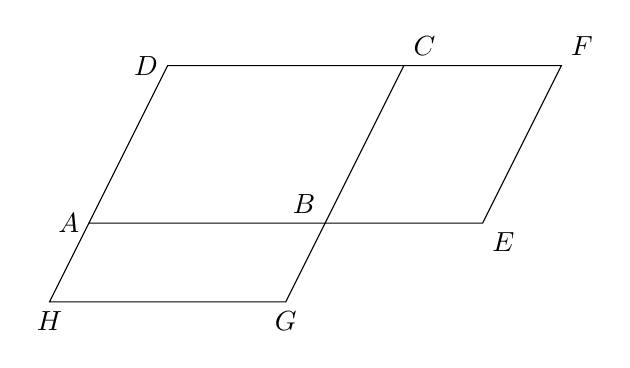
\begin{tikzpicture}
\coordinate (A) at (0,0);
\coordinate (B) at (3,0);
\coordinate (C) at (4,2);
\coordinate (D) at (1,2);
\coordinate (E) at (5,0);
\coordinate (F) at (6,2);
\coordinate (G) at (2.5,-1);
\coordinate (H) at (-0.5,-1);
\draw   (A) node[left] {$A$} -- 
        (B) node[above left] {$B$} --
        (C) node[above right] {$C$} --
        (D) node[left] {$D$} --
        cycle;
\draw   (B) --
        (E) node[below right] {$E$} --
        (F) node[above right] {$F$} --
        (C);
\draw   (B) --
        (G) node[below] {$G$} --
        (H) node[below] {$H$} --
        (A);
\end{tikzpicture}
\end{center}

\begin{subparts}
\subpart Donner deux vecteurs égaux à $\vect{AB}$.
\subpart Donner un représentant de $\vect{DA}$ d'origine $C$.
\subpart Donner un vecteur \textbf{opposé} à $\vect{GH}$.
\subpart Donner un vecteur colinéaire à $\vect{EF}$, \textbf{mais de norme différente}.
\end{subparts}
\end{parts}

\titledquestion{Somme de vecteurs}[5]
\begin{parts}
\part Soit $P, Q$ et $R$ trois points quelconques du plan. Expliciter la relation de Chasles sur les vecteurs $\vect{PQ}$ et $\vect{QR}$
\part Simplifier les expressions suivantes :
\begin{subparts}
\subpart $\vect{DC} + \vect{CA} = \dots$
\subpart $\vect{AC} + \vect{CI} + \vect{IJ} = \dots$
\subpart $\vect{GH} + \vect{FG} = \dots$
\subpart $\vect{XY} - \vect{XZ} = \dots$
\end{subparts}
\part Placer sur la figure suivante le vecteur $\vect{u} + \vect{v}$ et $\vect{u} - \vect{v}$.
\begin{center}
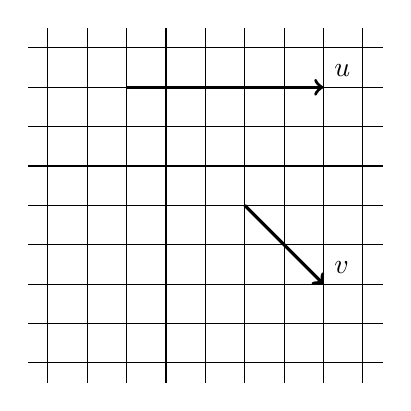
\begin{tikzpicture}
\draw (-2.25,-2.25) grid[step=0.5,help lines] (2.25,2.25);
\draw[very thick, ->] (-1,1.5) -- (1.5,1.5) node[above right] {$\vect{u}$};
\draw[very thick, ->] (0.5,0) -- (1.5,-1) node[above right] {$\vect{v}$};
\end{tikzpicture}
\end{center} 
\end{parts}
\newpage
\titledquestion{Colinéarité}[5]
\begin{parts}
\part Soient $\vect{u}$ et $\vect{v}$ deux vecteurs tels que il existe un nombre $k$ vérifiant $\vect{u} = k \times \vect{v}$. Que peut-on en déduire de $\vect{u}$ et de $\vect{v}$?
\part Soit $ABC$ le triangle suivant :
\begin{center}
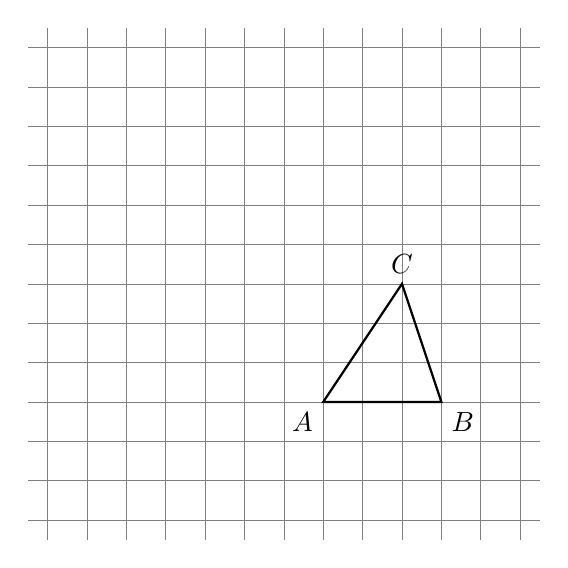
\begin{tikzpicture}
\coordinate (A) at (0.5,-1.5);
\coordinate (B) at (2,-1.5);
\coordinate (C) at (1.5,0);
\draw[help lines] (-3.25,-3.25) grid[step=0.5] (3.25,3.25);
\draw[thick]   
        (A) node[below left] {$A$} -- 
        (B) node[below right] {$B$} -- 
        (C) node[above] {$C$} -- 
        cycle;
\end{tikzpicture}
\end{center}
\begin{subparts}
\subpart Placer les points $D$ et $E$ vérifiant $\vect{AD} = 2\vect{BA}$ et $\vect{BE} = 3\vect{BC}$.
\subpart Justifier que $\vect{DE} = \vect{DA} + \vect{AB} + \vect{BE}$.
\subpart En déduire que $\vect{DE} = 3\vect{AC}$
\subpart Que peut-on en conclure pour les droites $(DE)$ et $(AC)$ ?
\end{subparts}
\end{parts}

\titledquestion{Démonstration}[5]
Soit $ABCD$ un quadrilatère quelconque. On pose quatre points $I,J,K$ et $L$ quatre points définis par 
\begin{equation*}
\begin{aligned}
\vect{AI} &= \dfrac{1}{2}\vect{AB}\\
\vect{BJ} &= \dfrac{1}{2}\vect{BC}\\
\vect{CK} &= \dfrac{1}{2}\vect{CD}\\
\vect{DL} &= \dfrac{1}{2}\vect{DA}\\
\end{aligned}
\end{equation*}
\begin{parts}
\part Tracer la figure correspondante \textbf{dans le cas où $ABCD$ est un carré}.
\part Justifier que $\vect{IJ} = \vect{IA} + \vect{AB} + \vect{BJ}$.
\part En déduire que $\vect{IJ} = \dfrac{1}{2}\vect{AB} + \dfrac{1}{2}\vect{BC}$.
\part En déduire une expression de $\vect{IJ}$ en fonction de $\vect{AC}$.
\part De la même manière, en partant de $\vect{LK}=\vect{LD} + \vect{DC} + \vect{CK}$ (pas besoin de le justifier), montrer que $\vect{LK}=\dfrac{1}{2}\vect{AD} + \dfrac{1}{2}\vect{DC}$.
\part En déduire une expression de $\vect{LK}$ en fonction de $\vect{AC}$.
\part Que peut-on en déduire du quadrilatère $IJKL$ ?
\end{parts}
\end{questions}
\end{document}